\chapter{Architektur}

\section{Übersicht}

Um die beschriebenen Funktionalen- und Nicht-Funktionalen Anforderungen erfüllen zu können haben wir die folgende Architektur entwickelt. \\

Um eine Drohne über einen Server in der Cloud steuern zu können, muss diese mit dem Internet verbunden werden. Um dies zu erreichen verwenden wir ein Smartphone, dass auf der Drohne angebracht wird und über USB mit dem Flight-Controller verbunden ist.  (siehe Abb. \ref{fig:architecture-overview}). Das Smartphone wird aber auch benötigt um dem Drone-Operator ein Benutzeroberfläche zur Verfügung zu stellen, die das Beladen und das Abfragen des Zustands der Drohne ermöglichen. \\

\begin{figure}[h]
	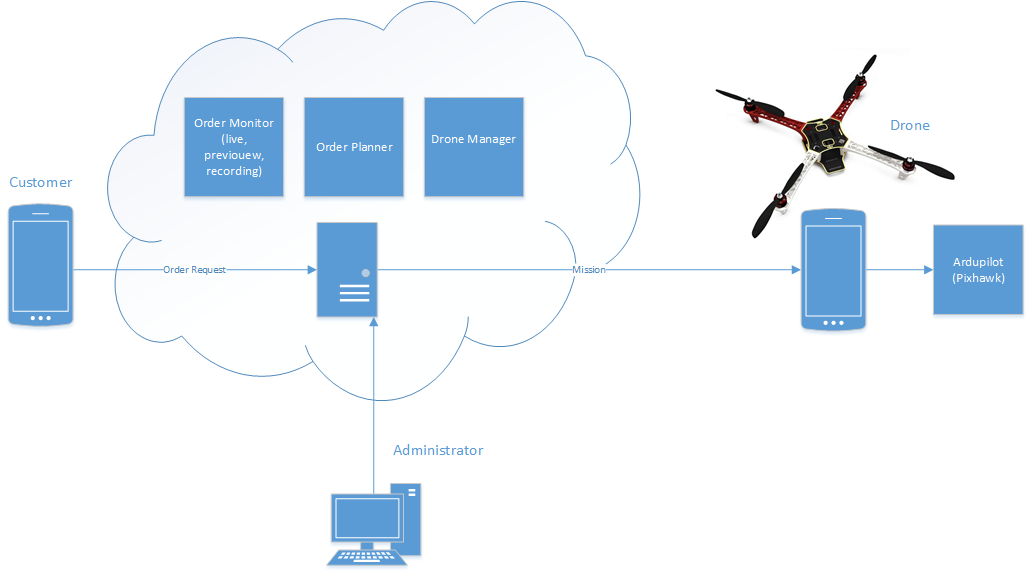
\includegraphics[width=1.0\textwidth]{images/Overview-Diagram.png}
	\caption{Übersicht der Project Helin Architektur }
	\label{fig:architecture-overview}
\end{figure}

\section{Kommunikations-Architektur}

Die Abbildung \ref{fig:communication-architecture-overview} zeigt die Kommunikations-Architektur in der Übersicht. Wichtig sind vor allem die verschiedenen verwendeten Protokolle, die benötigt werden um die Anforderungen erfüllen zu können. Bei den mobilen Geräten wird Messaging (AMQP) verwendet um bidirektionale Kommunikation zu ermöglichen. Dies ist nötig, damit Kunden und Administratoren die Bewegungen der Drohne live verfolgen können. 

Die eingesetzte Technologie für die Kommunikation zwischen dem Server und den Mobiltelefonen muss ausserdem den Nicht-Funktionalen-Anforderungen gerecht werden

Ausserdem bietet Messaging mit "Exactly Once" ein wichtiges Feature um die nötige Zuverlässigkeit zu gewährleisten. 


\begin{figure}[h]
	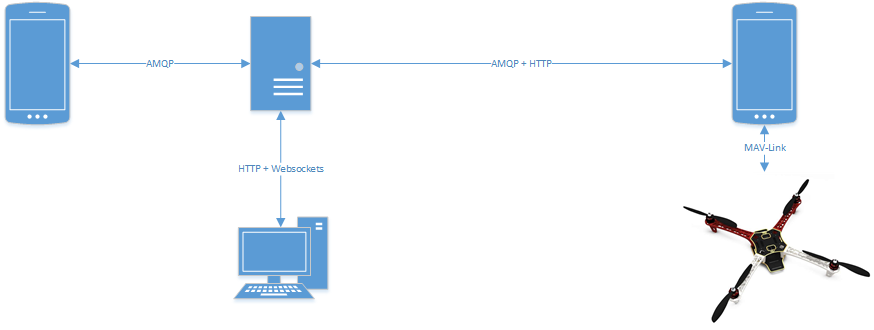
\includegraphics[width=1.0\textwidth]{images/Communication-Overview-Diagram.png}
	\caption{Übersicht der Kommunikations-Architektur mit den jeweiligen Protokollen. }
	\label{fig:communication-architecture-overview}
\end{figure}